\documentclass[../main.tex]{subfiles}
\graphicspath{{\subfix{../images/}}}
\begin{document}
 
  %TODO intro da fundamentacao
  O referencial teórico do projeto Caramelo consiste em uma síntese abordando as características de um robô quadrúpede - quanto ao design, os atuadores e os subsistemas de processamentos que podem ser utilizados. Além disso, é apresentado também sobre o planejamento dos movimentos de marcha e quanto ao controle de locomoção de robôs quadrúpedes, utilizando um modelo cinemático baseado nas considerações de Denavit-Hartenberg.

  \subsection{Apresentação e conceito geral}
  O robô quadrúpede é um sistema robótico móvel que se locomove com a ajuda de pernas. Robôs móveis podem ser divididos em três grupos, relacionados aos seus sistemas de locomoção: robôs com rodas, com esteiras e com pernas. Quando comparado aos dois primeiros, o último grupo apresenta diversas particularidades que o confere muitas vantagens quanto a mobilidade, robustez a diferentes terrenos e superação de obstáculos \cite{Biswal2021}. Robôs com rodas e esteiras apresentam boa performance em terrenos planos e conseguem navegar de forma autônoma pelo espaço, desde que haja um caminho contínuo entre os pontos de origem e destino. Robôs com pernas, por outro lado, são capazes de escolher os melhores pontos de suporte no terreno para apoiar seus pés, o que permite uma navegação em caminhos discretos (com obstáculos de grande inclinação e variação de altura) \cite{Yao2021}. Essa capacidade de se adaptar a terrenos desnivelados amplia bastante as oportunidades de aplicações às quais esse tipo de sistema pode ser designado: industriais, militares, missões de inspeção, resgate, entre várias outras. Por outro lado, essas vantagens vêm às custas de uma maior complexidade de controle e menor estabilidade.

  Robôs com pernas também apresentam diversas diferenças entre si, majoritariamente ligadas à quantidade de pernas que possuem. A quantidade de pernas de um robô está diretamente relacionada a sua estabilidade, capacidade de locomoção e eficiência. Os bípedes possuem baixa estabilidade, visto que se apoiam em apenas uma perna para poder andar. Os com múltiplas pernas (mais de quatro) possuem maior estabilidade, afinal conseguem manter pelo menos três (muitas vezes até quatro) pontos de apoio no solo enquanto realizam um passo. No entanto, cada perna representa um conjunto adicional de juntas e atuadores, diminuindo a eficiência do sistema como um todo. Os quadrúpedes conseguem unir vantagens desses dois tipos ao apresentar um balanço entre estabilidade e eficiência. Eles possuem uma estabilidade passiva quando estáticos, pois se apoiam em quatro pontos. Além disso, também são capazes de navegar de forma estável em baixas velocidade, movendo uma perna por vez enquanto as outras três permanecem no solo. Isso elimina a redundância presente nos robôs com múltiplas pernas, aumentando sua eficiência \cite{Yao2021}.

  \subsection{Estrutura e design}
  Pelo fato de robôs quadrúpedes terem se tornado um grande foco de pesquisa nos últimos anos, diferentes \textit{designs} já foram pesquisados, variando, por exemplo, estrutura, configuração de pernas e o número de graus de liberdade (GDL) por perna. 
  
  Um dos tipos de estrutura que existem é a de tipo mamífero. Dois exemplos de robôs que utilizam essa estrutura estão ilustrados na Figura \ref{fig:structure_design}. 

  %TODO adicionar figura dos planos frontal, sagital
  \begin{figure}
    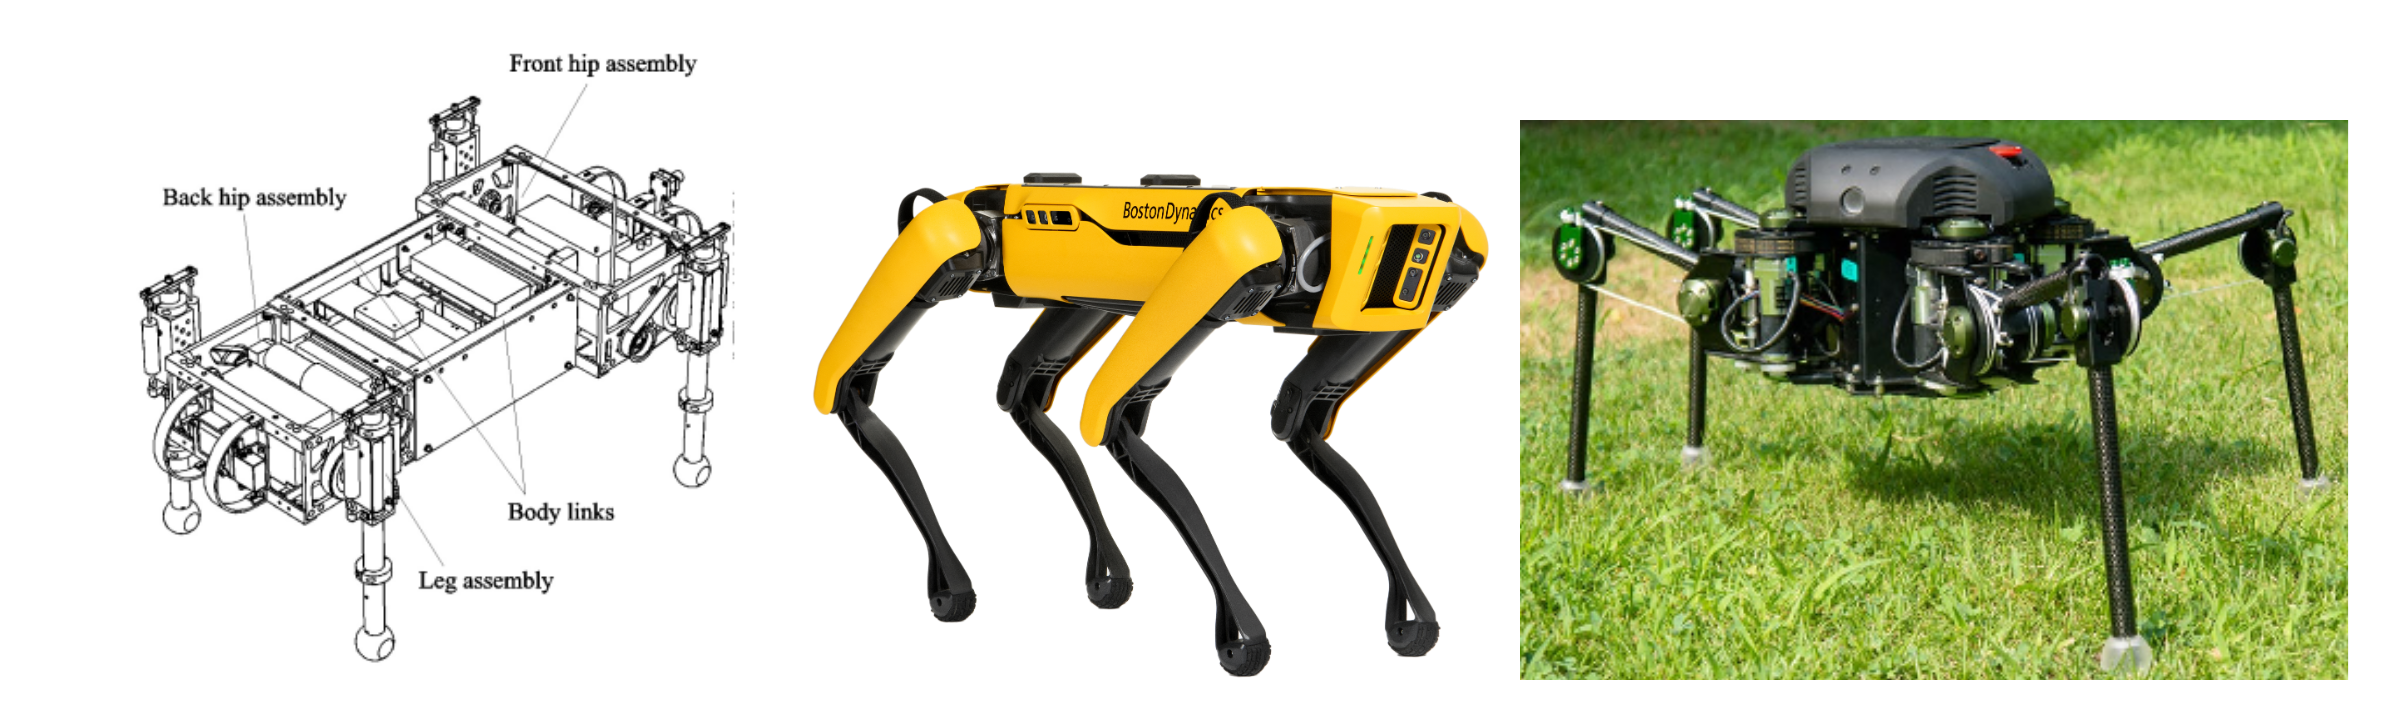
\includegraphics[width=0.48\textwidth]{structure_design.png}
    SCOUT-II / SPOT / TITAN-XIII
    \label{fig:structure_design}
  \end{figure}

  A estrutura tipo mamífero tem esse nome por conta da sua semelhança com a postura de mamíferos quadrúpedes como cachorros e cavalos. Kitano et al., em \cite{Kitano2016}, analisa dois tipos diferentes de estruturas de robôs quadrúpedes: a do tipo \textit{sprawling} e a do tipo mamífero. Segundo a análise, essa última permite alcançar maiores velocidades, por possuir duas juntas no plano sagital. Além disso, ela também é mais eficiente, pois os atuadores utilizam menos torque para sustentar o robô: sua estrutura mais compacta diminui o braço de alavanca sobre o qual a força peso do robô atua. Essa estrutura também favorece a navegação em ambientes estreitos, onde um robô do tipo \textit{sprawling}, por exemplo, teria dificuldades de acessar.

  A estrutura adotada nesse trabalho é a do tipo mamífero. Os robôs quadrúpedes que utilizam essa estrutura também se diferenciam quanto à configuração das pernas. Existem quatro tipos de configuração de pernas e elas estão ilustradas na Figura \ref{fig:joint_configurations}.
  
  \begin{figure}[h]
    \centering
    \caption{Titulo da Figura}
    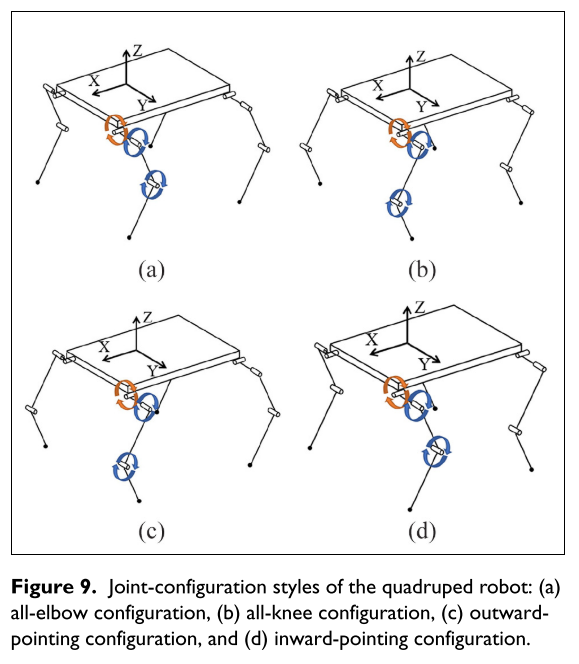
\includegraphics[width=0.48\textwidth]{joint_configurations.png}
    
    Fonte: XXX
    \label{fig:joint_configurations}
  \end{figure}

  Entre elas destacam-se a \textit{full-elbow} e o \textit{elbow-knee}. Robôs como o Spot, MIT Cheetah e Stanford Pupper utilizam a configuração \textit{full-elbow}, enquanto outros como o ANYmal, StarlETH e BigDog adotam a configuração  \textit{elbow-knee}. \textbf{\textcolor{red}{\textit{Yao et al.}}} acreditam que a configuração \textit{elbow-knee} possibilita maior estabilidade, mas as características de movimento da configuração \textit{full-elbow} podem ser superiores.

  O número de juntas nas pernas, que coincide com a quantidade de GDL do robô, também é um dos aspectos estudados sobre os quadrúpedes. A maioria apresenta 3 GDL por perna, o que é suficiente para que o robô consiga mover seus pés em três dimensões e realize diversos tipos de marchas. A fim de simplificar a estrutura e consequentemente o controle, alguns robôs utilizam apenas 2 GDL por perna, eliminando a junta no corpo que movimenta a perna no plano frontal. Outros robôs buscam performances mais semelhantes ao andar de animais reais, o que demanda maior flexibilidade de movimento, justificando o acréscimo de uma quarta junta. No entanto, como já mencionado, esse acréscimo aumenta a complexidade do controle e prejudica a eficiência. Essa perda de eficiência se dá porque mais atuadores significa mais consumo de energia e também mais massa. 
  
  A massa do robô quadrúpede deve ser a menor possível. Quanto mais leve for o sistema, menos torque será demandado dos motores e maior sua eficiência. Além disso, a distribuição de massa do robô também é um aspecto muito importante. A massa deve ser localizada majoritariamente no corpo, enquanto as pernas devem possuir baixa inércia. Isso permite que elas se movam rapidamente sem alterar, de forma significativa, o centro de gravidade do robô, o que aumenta a estabilidade e requer menos complexidade de controle. Possuir baixa inércia significa possuir baixa massa. Por outro lado, as pernas devem ser resistentes o suficiente para suportar o peso do robô, além de distúrbios causados pelo impacto dos pés com o chão, o que pode demandar um aumento de massa nas pernas. Um balanço entre massa e resistência deve ser buscado ao mesmo tempo em que deve-se buscar diminuir a massa total do sistema \cite{Zhong2019}.

  \subsection{Movimentação por marchas}
  Robôs quadrúpedes se movimentam conforme uma sequência de movimentos coordenados de suas pernas que compõe uma marcha. Em uma descrição mais detalhada, \textbf{\textcolor{red}{Song and Waldron (1989)}} afirma que: 

  \textcolor{red}{“Uma marcha é definida pelo tempo e local de colocação e levantamento de cada pé, coordenado com o movimento do corpo em seus seis graus de liberdade, para mover o corpo de um lugar para outro”.}
  
  Planejar a marcha de forma robusta é fundamental para garantir que um robô com pernas caminhe de forma eficiente e estável, especialmente em terrenos irregulares \cite{X.129}. Para isso, é necessário levar em consideração as etapas da marcha e, por consequência, seu tipo.
  
  Marchas são divididas em duas etapas: \textit{stance} e \textit{swing}. Durante a fase \textit{stance}, as pernas estão no solo e impulsionam o robô para frente. Na etapa de \textit{swing}, as pernas são erguidas para deslocar o pé até o próximo ponto de apoio. É importante ressaltar que as fases de \textit{stance} e \textit{swing} não ocorrem em todas as pernas ao mesmo tempo. A depender do tipo de marcha, algumas pernas podem estar em \textit{swing} enquanto outras estarão em \textit{stance}.

  O trot é um tipo de marcha muito utilizado por robôs quadrúpedes devido a sua simplicidade e eficiência. Este tipo de marcha é periódico e simétrico. Marchas periódicas são caracterizadas pelo fato de que os mesmos movimentos se sempre se repetem no mesmo instante dentro de um ciclo de locomoção \cite{de2006quadrupedal}. Já a simetria é uma característica de marchas que movimentam um par de pernas em conjunto, saindo e voltando para o solo de forma sincronizada. No trot, as pernas diagonais se movimentam em pares e quando um par está na etapa de \textit{swing} o outro está na etapa de \textit{stance}. Outra característica da marcha trot é que ela pode ser contínua ou descontínua. Uma marcha contínua mantém o corpo do robô em movimento constantemente, enquanto a descontínua submete o corpo a um movimento intermitente \cite{de2006quadrupedal}. Portanto, quando a marcha trot é contínua, as pernas em \textit{stance}, além de sustentar o robô, deslocam o corpo da direção do movimento, o que exige maior capacidade de controle. Em contrapartida, quando ela é descontínua o corpo fica estático esperando as pernas em \textit{swing} terminarem seu movimento para, então, ser deslocado quando as quatro pernas já estão no solo.

  \subsection{Controle de locomoção}
  \textcolor{red}{\textbf{TO-DO}
  \begin{itemize}
    \item Breve introdução ao tópico
  \end{itemize}
  }

  \subsubsection{Modelo cinemático}
  %TODO rever escrita: "variáveis de juntas", sintetizar "falar logo de junta rotational;
  Um modelo cinemático descreve a relação entre as variáveis de juntas e a posição e orientação do end-efector. Durante a análise cinemática de um robô quadrúpede, é afirmado que o sistema consiste de um corpo rígido composto por quatro pernas com três graus de liberdade \textbf{\textcolor{red}{[Fonte: p]}}. A fim de mover este corpo por uma dada trajetória, é necessário um movimento coordenado das juntas \textbf{\textcolor{red}{[q]}}. Logo, o modelo cinemático deve descrever a relação entre as variáveis de juntas e a posição do pé e suas derivadas. Considerando que as juntas são rotacionais, a variável de junta é definida como o ângulo entre os elos ligados por tal junta.

  O modelo cinemático de um corpo articulado em malha aberta pode ser dividido em dois problemas: cinemática direta e cinemática inversa. Durante a análise de cinemática direta, as variáveis das juntas fornecem a posição do \textit{end-efector}, enquanto que a cinemática inversa é o processo de encontrar os valores das juntas a partir da posição e orientação do \textit{end-efector}. Para mover o pé do robô quadrúpede até uma posição desejada, é necessário determinar os valores rotacionais das juntas das pernas com análise de cinemática inversa.
  
  %TODO rever writing
  A análise da cinemática inversa é frequentemente realizada por meio de métodos analíticos, como em \textbf{\textcolor{red}{[Fonte: p]}}, mas uma abordagem geométrica também pode ser aplicada. As equações que expressam a posição angular das juntas são não lineares e podem fornecer resultados impossíveis fisicamente. Além disso, também pode haver redundância de respostas, quando mais de um conjunto de posições dos pés fornecem a mesma posição final das juntas \textbf{\textcolor{red}{[Fonte: p]}}.

  Para a análise da cinemática direta, muitos autores utilizam os parâmetros de Denavit-Hartenberg. No desenvolvimento desse trabalho, foi utilizado o pacote \textit{TF2} do \textit{framework} ROS2 para obter os dados de cinemática direta.

  \subsubsection{Etapas do controle e conceitos gerais}
  A locomoção de robôs quadrúpede, em geral, segue uma sequêcia de passos. Essa sequência depende fortemente do design do robô e do tipo de marcha que será utilizada. Raibert propôs em \cite{Raibert1986} um método de controle baseado em três etapas: controle de salto, controle de velocidade e controle de postura do corpo. Essa pesquisa foi desenvolvida com robôs de pernas rígidas, semelhantes ao SCOUT-II, que utilizavam uma junta prismática nas pernas e uma rotativa junto ao corpo. Esse sistema de controle baseava-se na implementação independente de três controladores que, agindo em conjundo, controlam a locomoção do robô de forma estável, a partir da velocidade, da altura de salto do robô e do ângulo do corpo. Essa estratégia de controle foi utilizada para controlar robôs com uma, duas e quatro pernas, tanto no espaço 2D quanto 3D. Sua premissa básica era a de que apenas uma perna estaria em \textit{\textit{stance}} ou em \textit{\textit{swing}} por vez. A fim da satisfazer essa premissa para robôs com mais de duas pernas, foi proposto o conceito de pernas virtuais. Isto é, um conjunto de pernas deve realizar igual comportamento quando em \textit{\textit{swing}} e \textit{\textit{stance}} e as fases de \textit{swing} e \textit{stance} de cada conjunto devem ser alternadas. Dessa forma, é possível modelar o robô como possuindo apenas duas pernas virtuais, cada uma representando um dos dois conjuntos de pernas físicas em igual movimento. Tratando-se do quadrúpede, essa premissa pode ser satisfeita considerando duas pernas como uma perna virtual. O ponto de conexão dessa perna virtual no corpo do robô é localizado no centro da reta unindo ambos os pontos de conexão com o corpo das pernas físicas. Utilizando esse conceito, pode-se utilizar marchas simétricas como o \textit{trot}, \textit{pace} e \textit{bound}.

  A estratégia de controle em três etapas proposta por \textcolor{red}{Raibert} foi responsável por locomover robôs com pernas rígidas de maneira simples, porém esses robôs não tinham autonomia de energia (eram alimentados por um capo umbilical a uma fonte externa) e apenas operavam no terreno plano e controlado do laboratório. A fim de possibilitar a operação de robôs com pernas em terrenos desnivelados e de difícil mobilidade, os robôs quadrúpedes passaram por modificações de design e estratégias de controle. Outro marco nessa área de pesquisa foi o robô BigDog, cujo trabalho foi publicado por \textbf{\textcolor{red}{Raibert et al.}} \textbf{\textcolor{red}{[Fonte: BigDog, the Rough-Terrain Quadruped Robot]}}. O BigDog é um robô quadrúpede com 4 GDL por perna movido por atuadores hidráulicos. Essa maior flexibilidade de movimentação das pernas permite controlar a locomoção do robô sem que este precise saltar, sendo possível, então, dividir o controle de locomoção em duas etapas principais: controle de \textit{stance} e controle de \textit{\textit{swing}}. Assim, a velocidade do robô, postura do corpo e altura do corpo em relação ao chão, que é equivalente ao controle de altura do salto, seriam estados controlados por esses dois controladores, o de \textit{\textit{stance}} e o de \textit{\textit{swing}}.

  O controlador de \textit{stance} é responsável por controlar o comportamento das pernas na fase de \textit{stance}, quando as pernas devem utilizar a tração com o terreno para manter o corpo em equilíbrio e direcioná-lo na direção desejada de locomoção. Enquanto isso, o controlador de \textit{\textit{swing}} é responsável por controlar as pernas em \textit{swing}, de forma que os pés (\textit{end-effectors}) sigam a trajetória de um passo até o próximo ponto de apoio no chão. Para robôs quadrúpedes, ambos os controladores operam simultaneamente, porém em pernas diferentes, seguindo o princípio, muitas vezes, das pernas virtuais. O componente do sistema de controle responsável por coordenar as fases de cada perna é o planejador de marchas (\textit{gait planner} ou \textit{gait scheduler}).

  Como cada perna se comporta durante cada fase é algo que varia com o método de controle utilizado por cada robô, mais ainda é possível elencar semelhanças gerais. Na fase de \textit{\textit{swing}}, calcula-se o local do próximo ponto de apoio dos pés, com base na velocidade desejada para o robô, e uma trajetória de passo até esse ponto. Essa trajetória pode ser uma curva senoidal \cite{X.118}, triangular \textbf{\textcolor{red}{[Fontes: github.com/mike4192/spotMicro /stanfordroboticsclub/StanfordQuadruped]}}, de Bezier \textbf{\textcolor{red}{[Fonte: hackaday.io/project/171456-diy-hobby-servos-quadruped-robot]}}, cicloidal \cite{Shi2021} \cite{X.58}, entre outras, e o componente encarregado por calculá-la é o planejador de trajetórias. Uma consideração comum é a de que as trajetórias das pernas em cada fase são independentes, de tal forma que o estado do pé no momento em que toca o solo se torna um dos pontos chave para a estabilidade do robô  \cite{X.118}. Nesse sentido, a trajetória cicloidal ganha destaque, porém outras curvas podem ser utilizadas para gerar diferentes perfis de aceleração e velocidade dos pés durante uma passada. Curvas como a de Bezier, por exemplo, possuem grande flexibilidade, o que permite se criar várias trajetórias distintas que podem ser geradas em tempo-real, como é feito em  \textbf{\textcolor{red}{[Fonte: Dynamics and Domain Randomized Gait Modulation with Bezier Curves for Sim-to-Real Legged Locomotion]}}.

  Já na fase de \textit{\textit{stance}}, as pernas devem manter o robô em equilíbrio ao mesmo tempo que direcionam o corpo na direção de locomoção desejada. Para isso, alguns trabalhos utilizam trajetórias de um formato fixo para os pés, assim como na fase de \textit{\textit{swing}}, porém, não necessariamente com o mesmo formato de curva usado nesta última \cite{X.118} \cite{X.58}. Além disso, controladores de equilíbrio também podem ser implementados. Esses controladores visam estabilizar o pitch e roll do robô \cite{Shi2021} \textbf{\textcolor{red}{[Fontes:hackaday.io/project/171456-diy-hobby-servos-quadruped-robot, StanfordQuadrupedm notspot-sim-cpp ]}} ou até mais graus de liberdade, como em \cite{Chen2020140736} \cite{X.134} \cite{Zhang2016284}. Eles podem ser baseados na leitura de sensores inerciais ou no equilíbrio das forças de contato com o solo que atuam em cada perna, por exemplo.


  \subsubsection{Método de controle}
  %TODO REVISAR e REDUZIR
  Os métodos apresentados anteriormente baseiam-se ou em um modelo dinâmico para o sistema ou na dinâmica de componentes mecânicos arbitrários. Contudo, é possível alcançar boa performance de locomoção utilizando, também, todo o sistema em malha aberta, como é feito em [X]. Nesse caso, é implementado um controle de posição nas juntas do robô - diferente dos métodos mencionados anteriormente, que costuma se basear no controle de torque - e um controlador de alto nível cacula a posição de cada junta no tempo com base na fase de cada perna, na trajetória que elas devem seguir, no período escolhido para o passo e na cinemática inversa do robô e envia o sinal para o atuador. Esse método de controle de locomoção é bastante simples e fácil de implementar. Ele é aplicado, especialmente, em robôs de pequeno porte, atuados por servomotores e com baixa capacidade de processamento. No entando, em terrenos até pouco desnivelados, as pernas irão, eventualmente, perder sincronia e o robô irá tombar.

  Uma maneira de melhorar a performance é fechando a malha de controle, tanto da fase de *\textit{stance}* quanto da fase de *\textit{swing}*. Na fase de *\textit{swing}*, o *feedback* de posição das juntas, aplicado à cinemática direta, pode fornecer a atual posição do pé, permitindo um controle mais robusto do passo e uma maior sincronia entre as pernas. Já na fase de *\textit{stance}*, a angulação do corpo do robô  pode ser usada para corrigir sua postura (roll, pitch e yaw), com o auxílio de controladores baseados em PID, como feito em [X]. O controle de postura cumpre o papel de corrigir distúrbios tanto internos do sistema, como deslocamentos do centro de massa oriundos da movimentação das pernas em *\textit{swing}*, quanto externos, frutos de uma colisão com outros corpos ou de desníveis no terreno. Além de corrigir distúrbios, o controle de postura também pode ser usado para manter o corpo do robô numa angulação paralela à superfície de locomoção, seja esta plana ou inclinada, o que ajuda a aumentar a estabilidade de robô. Chen *et al.* em [X], utilizaram essa correção junto com o controle de altura do COM como uma das etapas do seu controlador anti-distúrbios e mostraram como ela ajuda a distribuir melhor a força entre as pernas em *\textit{stance}* e aumentar o espaço de trabalho das pernas, principalmente quando em superfícies inclinadas.

  \subsection{Projeto do robô}
  
\end{document}
